\documentclass[]{article}

\usepackage[margin=1.0in]{geometry}
\usepackage{amsmath}
\usepackage{amsfonts}
\usepackage{amsthm}
\usepackage{graphicx}
\usepackage{amssymb}

\usepackage{mathtools}

%opening
\title{Project Overview}
\author{Alex Karlovitz}
\date{}

\begin{document}
	
	\maketitle
	
This document contains a brief overview of my thesis project. 
The task is to extend Hejhal's algorithm for computing the Fourier coefficients and Laplace eigenvalues of Maass forms to a more general situation.
\\

\textbf{Goals:}
\begin{itemize}
	\item To compute the Hausdorff dimension of the Appolonian circle packing to high precision
	\begin{itemize}
		\item The Appolonian circle packing can be recognized as the limit set of a group action on hyperbolic 3-space
		\item There is a relationship (due to Patterson-Sullivan) between the Hausdorff dimension of a limit set and the base eigenvalue of the Laplace operator
	\end{itemize}
	\item To extend Hejhal's algorithm to work in hyperbolic 3-space
\end{itemize}

\textbf{Strategy:}
\begin{itemize}
	\item[$\checkmark$] Review previous work done by Kontorovich and Str\"ombergsson which extends Hejhal's algorithm to infinite volume fundamental domains (in hyperbolic 2-space)
	\item Modify K-S's algorithm so that it does not use the cuspidal expansion (since there is no appropriate analog of this in hyperbolic 3-space)
	\item Extend the new algorithm to work in 3 dimensions
	\item Apply the new algorithm to the Appolonian case
\end{itemize}

\section*{Algorithm Setup}

We have been using Hecke triangle groups as an example for testing.
The Hecke triangle group $\Gamma_r$ is the one-parameter subgroup of $\text{SL}(2, \mathbb{R})$ defined by
$$
\Gamma_r = \left\langle
	\begin{pmatrix}
		1 & 1 \\
		0 & 1
	\end{pmatrix},
	\begin{pmatrix}
		0 & -r \\
		\frac{1}{r} & 0
	\end{pmatrix}
\right\rangle
$$
We are interested in computing the base eigenvalue $\lambda$ for the action of the differential operator $\Delta$ acting on $L^2(\Gamma_r\backslash\mathbb{H})$.

\textbf{Note:} we will often use $s$ or $\nu$ when referring to the base eigenvalue; these are defined by
$$
\lambda = s(1 - s) ~~~~~~~~ \nu = \frac{1}{2} - s
$$

To get our hands on some data, we use Fourier expansions of the base eigenfunction.
We have three methods of getting an expansion.
First, since automorphic functions are invariant under $z \mapsto z + 1$, we have an expansion in the $x$-variable:
$$
f(x, y) = \sum_{n \in \mathbb{Z}}a_nW_n(y)e(nx)
$$
We could also conjugate our group so that it contains a non-identity diagonal element.
Since this causes automorphic functions to be invariant under the map $z \mapsto \kappa z$ for some $\kappa > 1$, we get a logarithmic Fourier expansion in the $\rho$-variable where $(\rho, \theta)$ denotes polar coordinates on $\mathbb{H}$:
$$
g(\rho, \theta) = \sum_{n \in \mathbb{Z}}b_nW_n^{(f)}(\theta)e\left( n\frac{\log\rho}{\log\kappa} \right)
$$
Finally, we could use a Cayley transform to take $\mathbb{H}$ to $\mathbb{D}$.
Functions on the disk are automatically invariant under $\theta \mapsto \theta + 2\pi$, so the base eigenfunction - written in polar coordinates on the disk - will have a Fourier expansion in the $\theta$-variable:
$$
h(\rho, \theta) = \sum_{n \in \mathbb{Z}}c_nW_n^{(d)}(\rho)e^{in\theta}
$$
More details on the Whittaker functions $W_n, W_n^{(f)}$, and $W_n^{(d)}$ are given below.
\\

\textbf{Note:} although this is not made explicit in the notation, all three Whittaker functions are dependent on the eigenvalue $\lambda$, which is of course an unknown.

\section*{The Algorithm}

The basic idea of Hejhal's algorithm is that \textit{given the eigenvalue} $\lambda$, we could set up a linear system to solve for the Fourier coefficients $a_n, b_n$, or $c_n$ (or a combination thereof).
\\

Two problems immediately come to mind:
\begin{enumerate}
	\item We don't know the eigenvalue $\lambda$.
	\item We cannot input an infinite Fourier expansion into a computer.
\end{enumerate}
To rectify the second problem, we choose a cutoff $M$ and only use terms in the expansions with $|n| \leq M$ (when we use multiple expansions, we may use different cutoffs for each expansion).
The algorithm proceeds by guessing values of $\lambda$, then attempting to step towards the true eigenvalue.

\subsection*{The Linear System}

For a fixed test point $z$ in $\mathbb{H}$ (or $\mathbb{D}$), we have two methods of obtaining a linear equation for the Fourier coefficients:
\begin{enumerate}
	\item Take another point $z^*$ in the orbit of this test point, then set a Fourier expansion to be equal when evaluated at $z$ and at $z^*$.
	\begin{itemize}
		\item The base eigenfunction is equal at these two points by automorphy.
		\item We will often take test points outside of a fixed fundamental domain, then choose their pullback as the other point in the orbit.
	\end{itemize}
	\item Set two different Fourier expansions equal to each other, both evaluated at $z$.
\end{enumerate}
If we choose enough distinct test points, we will have more equations than variables.
Then we can use least squares (or a similar method) to solve for the Fourier coefficients of interest.

\subsection*{Iteration of the Eigenvalue}

Let us fix two sets of test points $\vec{z}_1$ and $\vec{z}_2$.
Using a guess $\lambda = s(1 - s)$ for the eigenvalue, we can set up a linear system as described above using the first set of test points, and solve for the Fourier coefficients.
Put these in a vector $\vec{v}_1(s)$.

\textbf{Note:} the coefficients $\vec{v}_1(s)$ will not be the exact coefficients; this is because the value of $s$ is just a guess, and because the expansions are computed only to a finite cutoff.

We can then do the same process using the second set of test points to get a nother vector of coefficients $\vec{v}_2(s)$.
Finally, we define the function
$$
E(s) = ||\vec{v}_1(s) - \vec{v}_2(s)||_2
$$
Note that $E(s) \approx 0$ when $\lambda = s(1 - s)$ is the true eigenvalue.
So we can employ any method (like the secant method or a grid search) to try to find the zero of this function $E(s)$.

\section*{The Whittaker Functions}

The base eigenfunction $f$ is an eigenfunction of the hyperbolic Laplace operator $\Delta$.
By applying the equation
$$
\Delta f + \lambda f = 0
$$
to the Fourier expansion of $f$, we can solve a differential equation for the Fourier coefficients.
In all three of our expansions, the Fourier coefficient ends up being a constant times a Whittaker function which depends on $\lambda$ and the other variable.

\subsection*{Cuspidal Expansion}

In $\mathbb{H}$, the hyperbolic Laplacian is
$$
\Delta = y^2\left( \frac{\partial^2}{\partial x^2} + \frac{\partial^2}{\partial y^2} \right)
$$
and the Whittaker function solving the differential equation is
$$
W_n(y) =
\begin{cases}
	y^{1 - s} & n = 0 \\
	\sqrt{y}K_\nu(2\pi|n|y) & n \neq 0
\end{cases}
$$
where $K_\nu$ is the $K$-Bessel function.

\subsection*{Flare Expansion}

In $(\rho, \theta)$ coordinates on $\mathbb{H}$, the hyperbolic Laplacian is
$$
\Delta = \sin^2\theta\left(r^2\frac{\partial^2}{\partial r^2} + r\frac{\partial}{\partial r} + \frac{\partial^2}{\partial\theta^2}\right)
$$
and the Whittaker function solving the differential equation is
$$
W_n^{(f)}(\theta) = \sqrt{\sin\theta}P^{-\nu}_{\mu_n}(\cos\theta)
$$
where
$$
\mu_n = -\frac{1}{2} + \frac{2\pi in}{\log \kappa}
$$
and $P_\mu^{-\nu}$ is the associated Legendre function of the first kind.

\subsection*{Disk Expansion}

In $(\rho, \theta)$ coordinates on $\mathbb{D}$, the hyperbolic Laplacian is
$$
\Delta = \frac{(1 - \rho^2)^2}{4}\frac{\partial^2}{\partial\rho^2} +
\frac{(1 - \rho^2)^2}{4\rho}\frac{\partial}{\partial\rho} +
\frac{(1 - \rho^2)^2}{4\rho^2}\frac{\partial^2}{\partial\theta^2}
$$
and the Whittaker function solving the differential equation is
$$
W_n^{(d)}(\theta) = (1 - \rho^2)^s\rho^{|n|} \prescript{}{2}{F}_1(s, s+|n|, 1+|n|; \rho^2)
$$
where $\prescript{}{2}{F}_1$ is a hypergeometric function.

\subsection*{Computing the Special Functions}

We compute the $K$-Bessel function using PARI's built-in function ``besselk.''
\\

We compute the hypergeometric function $\prescript{}{2}{F}_1(a, b, c; x)$ using its power series definition as given in Gradshteyn-Ryzhik, 9.100.
We sum up to and including the $z^N$ term.
$N$ is chosen using a heuristic method: stop when $p$ (the next term being added) has decreased in value at least 10 times in a row and
$$
|p| < \text{(current PARI precision)}*|x|
$$

We compute the Legendre-$P$ function using the formula Gradshteyn-Ryzhik 8.704, which relates it to the hypergeometric function.

\section*{Decay Rates of the Fourier Coefficients}

Next, we list results on how quickly the Fourier coefficients decay in the three expansions.
This allows us to choose the cutoff $M$ with an accurate idea of the error in taking a finite expansion.

For proofs of the following bounds, see fourierAsymptotics.pdf.

\subsection*{Cuspidal Expansion}

It can be shown that $K_\nu(Y)$ decays exponentially as $Y \rightarrow \infty$.
On the other hand, we show that
$$
|a_n| \ll_f n^{\delta-1/2}
$$
(I think there is a result that in fact, $|a_n| = O(1)$, where the implied constant depends on $f$; this appears to be true experimentally).
So, the entire Fourier coefficient
$$
a_n\sqrt{y}K_\nu(2\pi|n|y)
$$
decays exponentially with $n$.
In particular, once $n \approx 1/y$, the coefficients will begin to decay very quickly.

\subsection*{Flare Expansion}

It can be shown that
$$
b_n \ll |n|^se^{-\pi |n|\alpha/\log\kappa}
$$
where $\alpha$ is chosen so that the flare
$$
\{ re^{i\theta} : 1 < r < \kappa, 0 < \theta < \alpha \}
$$
is entirely contained in a single fundamental domain for $\Gamma\backslash\mathbb{H}$.
On the other hand, one finds that
$$
P_{\mu_n}^{-\nu}(\cos\theta) \sim (\sin\theta)^{-1/2}|n|^{-\nu-1/2}e^{2\pi|n|\theta/\log\kappa}
$$
Thus the entire Fourier coefficient
$$
b_n\sqrt{\sin\theta}P_{\mu_n}^{-\nu}(\cos\theta)
$$
decays exponentially as $n \rightarrow \infty$ so long as $\theta < \frac{\alpha}{2}$.
\\

\textbf{To Do:} think about this! I don't think I'm forcing $\theta < \alpha/2$ in the code!

\subsection*{Disk Expansion}

In the course of the proof in fourierAsymptotics.pdf, we find that
$$
|c_nW_n^{(d)}(\rho)| \leq c_0W_0^{(d)}(\rho)
$$
for all $\rho$ and $n$.
This is a nice, quick test to see if the code is acting as we think it should.

We also show that
$$
W_n^{(d)}(\rho) \sim \rho^{|n|}
$$
Plugging this into the previous equation, we see that
$$
c_n \ll \rho^{-|n|}
$$
as $n \rightarrow \infty$.
Now, this was true for any $\rho \in [0, 1)$.
The idea now is to take $\rho = 1 - \delta$, with $\delta > 0$ small.
Then for any $\rho < 1 - \delta$, the entire Fourier coefficient has exponential decay:
$$
c_nW_n(\rho) \ll \left( \frac{\rho}{1 - \delta} \right)^{|n|}
$$
Thus, inside any fixed radius $\rho \leq P$, there is a constant $M$ so that taking the finite Fourier expansion $|n| \leq M$ gives a good approximation to the Maass form.
\\

\textbf{Question:} can I take $\rho \rightarrow 1$ in the bound on $c_n$? I think the answer is no... Think about this!

\section*{Facts about the Base Eigenfunction}

Here, we list a few facts about the base eigenfunction which allow us to reduce the number of computations.
For proofs of these facts, see baseEigenfunc.pdf.
\\

Facts:
\begin{itemize}
	\item the base eigenfunction is real-valued and non-negative
	\item in the upper half plane model, the base eigenfunction $f(x + iy)$ is even in $x$
	\item in all three expansions, the constant part of the Fourier coefficients are real-valued
\end{itemize}

Using the above facts, it is a simple argument to show that we can ``fold'' the Fourier expansions to only have nonzero coefficients for nonnegative $n$.
Moreover, if we choose the Cayley transform from $\mathbb{H} \rightarrow \mathbb{D}$ to force automorphic functions to be invariant under $w \mapsto -w$, we can take the odd coefficients in the disk expansion to be $0$.
\\

Here are the new expansions.
\\

Cuspidal expansion.
$$
f(x + iy) = \sum_{n = 0}^{\infty}a_nW_n(y)\cos(2\pi nx)
$$

Flare expansion.
$$
g(r, \theta) =
\sum_{n=0}^{\infty}b_nW_n^{(f)}(\theta)\cos\left( 2\pi n\frac{\log r}{\log\kappa} \right)
$$

Disk expansion.
$$
h(\rho, \theta) = \sum_{n = 0}^{\infty}a_{2n}W_{2n}^{(d)}(\rho)\cos(2n\theta)
$$

\section*{Choosing Test Points}

From playing around with Str\"ombergsson's code (which uses the cuspidal and flare expansions together), it has become clear that the choice of test points is very important to the success of the algorithm.

Some heuristics to keep in mind when choosing test points:
\begin{itemize}
	\item For a given test point, we only want to use a specific Fourier expansion if it converges quickly at that point.
	\item We need to be careful that there are no redundancies between test points.
	Technically, if we have many more points that the number of coefficients we are solving for, the least squares won't care about the redundancies; but of course that would increase the number of computations unnecessarily.
	\begin{itemize}
		\item Obvious example: two test points in the same orbit.
		\item Example: evenness plus invariance under $x \mapsto x + 1$ in the cuspidal expansion causes invariance under reflection across the line $x = \frac{1}{2}$.
		\item Similar examples occur in the flare and disk models.
	\end{itemize}
\end{itemize}

\subsection*{Pictures of Fundamental Domains}

\begin{figure}[h]
	\centering
	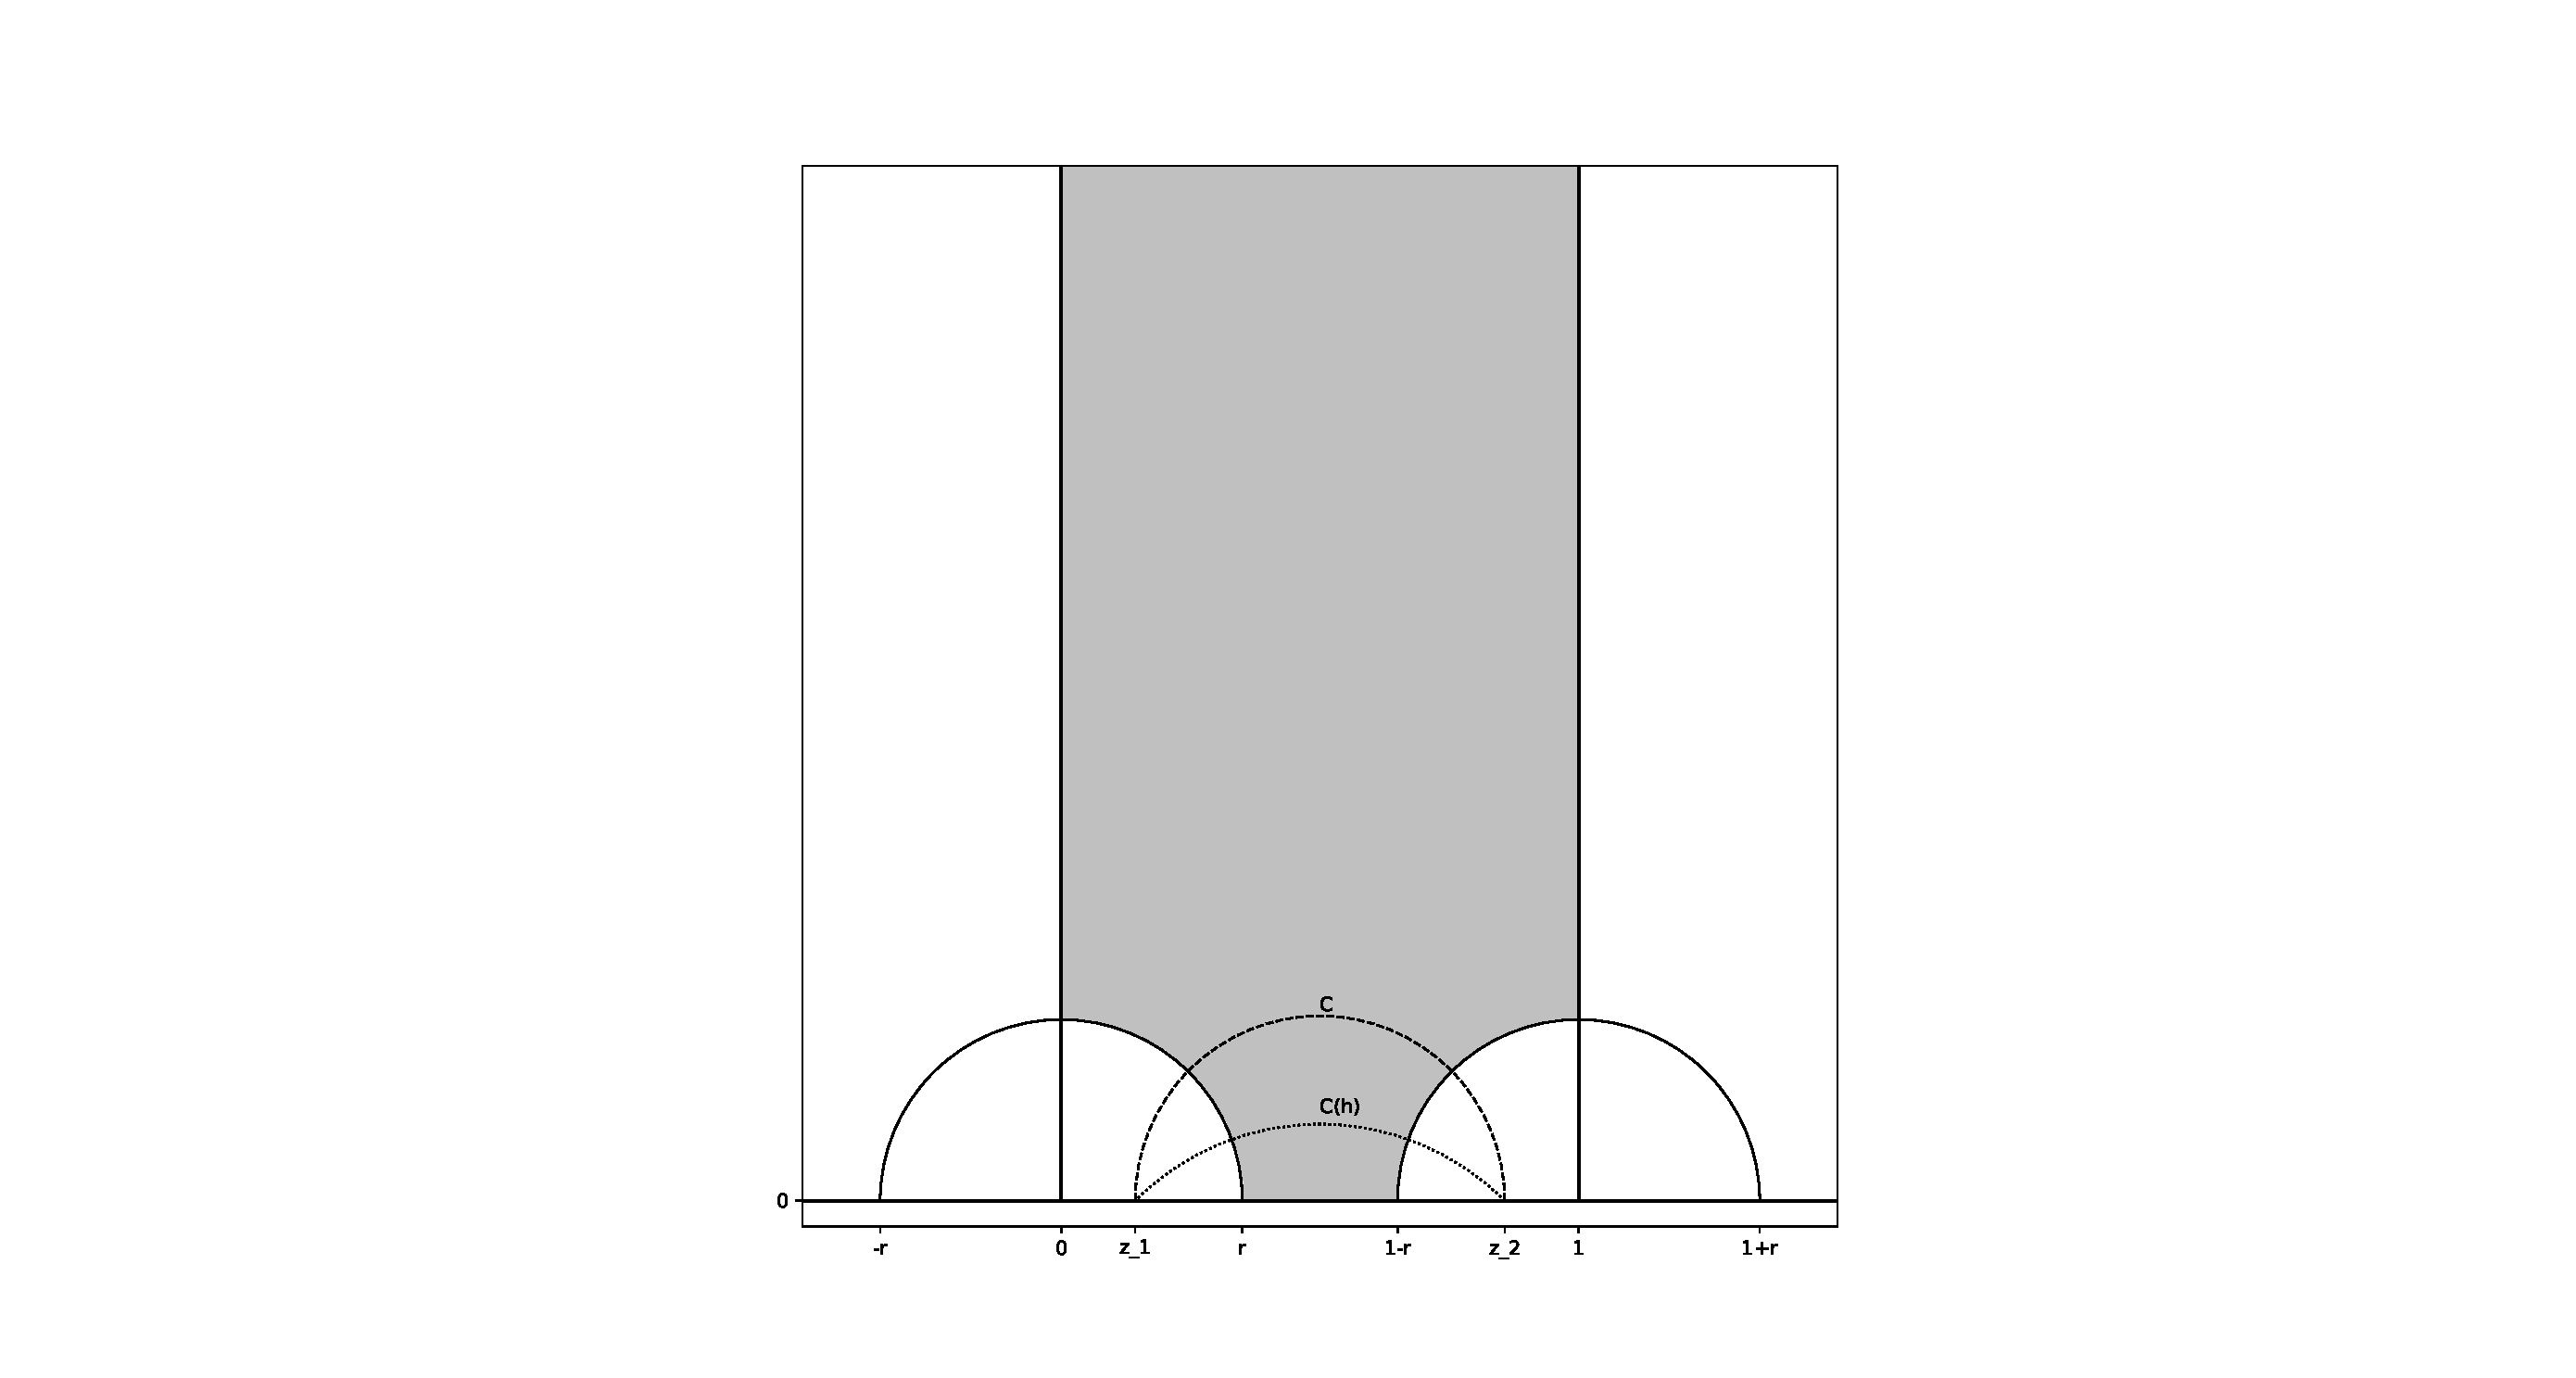
\includegraphics[trim=400 60 380 80, clip, width=0.6\linewidth]{F_r_with_Cs.pdf}
	\caption{$\mathcal{F}_r$ for $r = 7/20$ with $C$ and $C(h)$ for some $h > 0$}
	\label{FrWithCs}
\end{figure}

\begin{figure}[h]
	\centering
	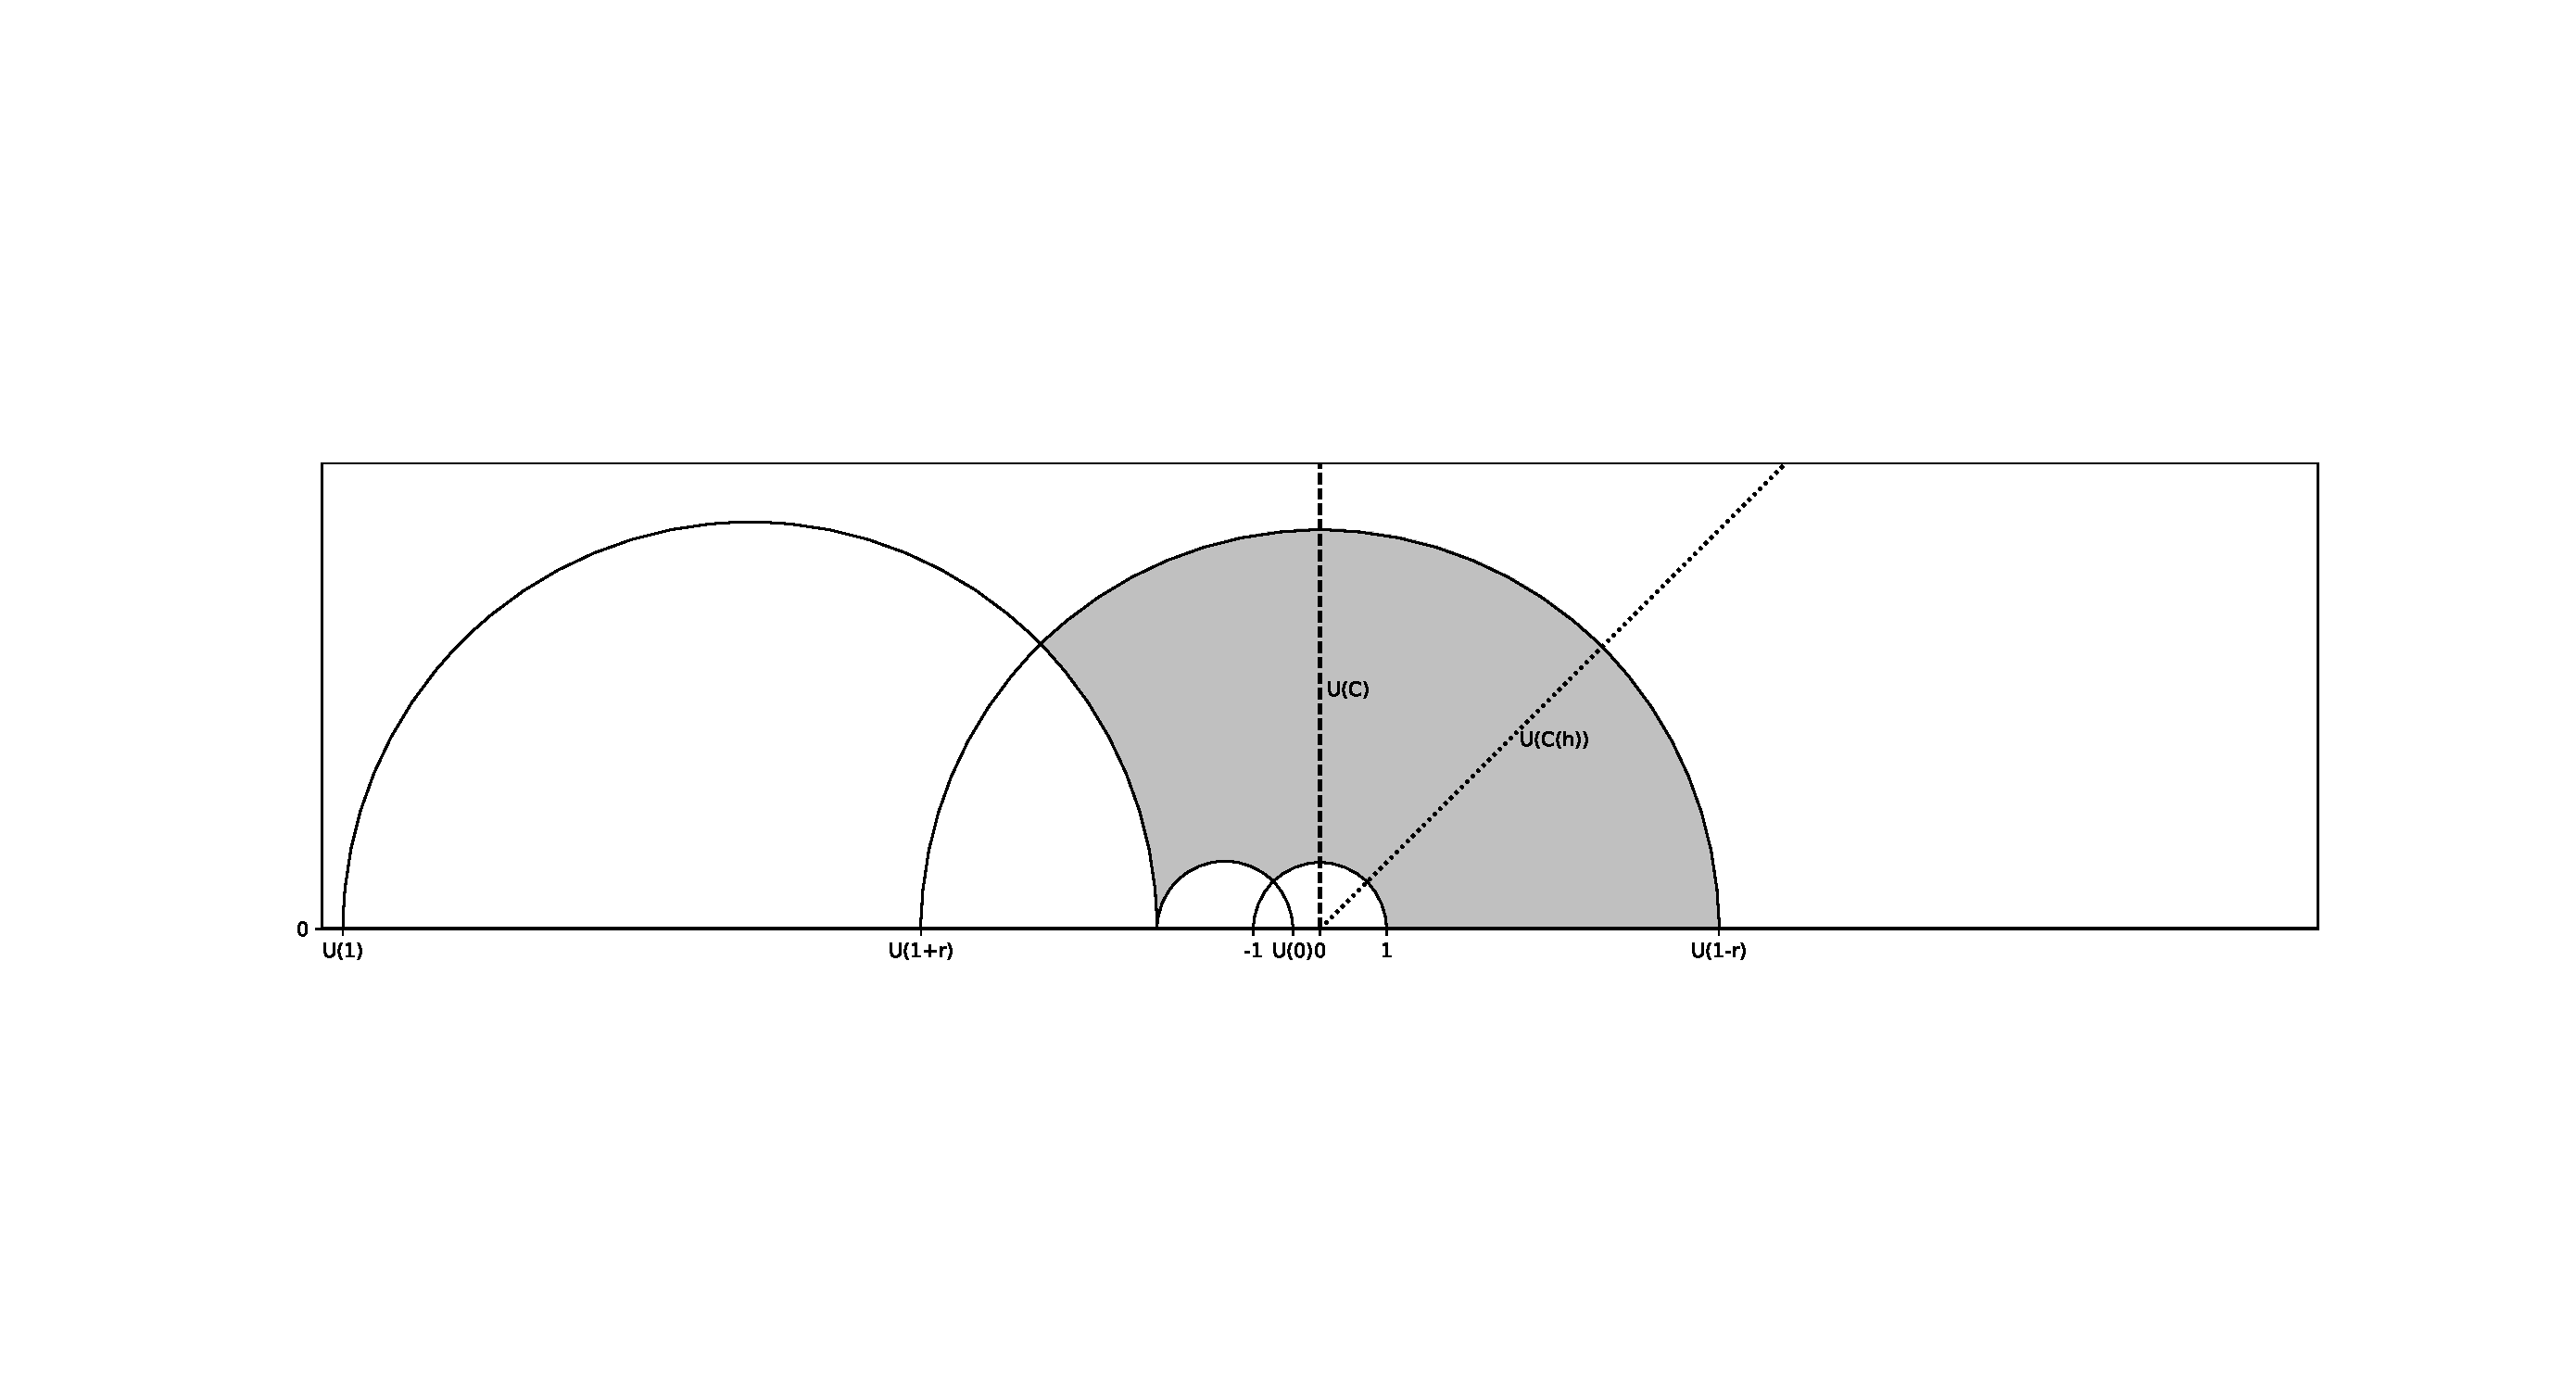
\includegraphics[trim=150 210 130 230, clip, width=\linewidth]{U_F_r.pdf}
	\caption{$U(\mathcal{F}_r)$ with $\mathcal{F}_r$ as in Figure \ref{FrWithCs}}
	\label{UFr}
\end{figure}

\begin{figure}[h]
	\centering
	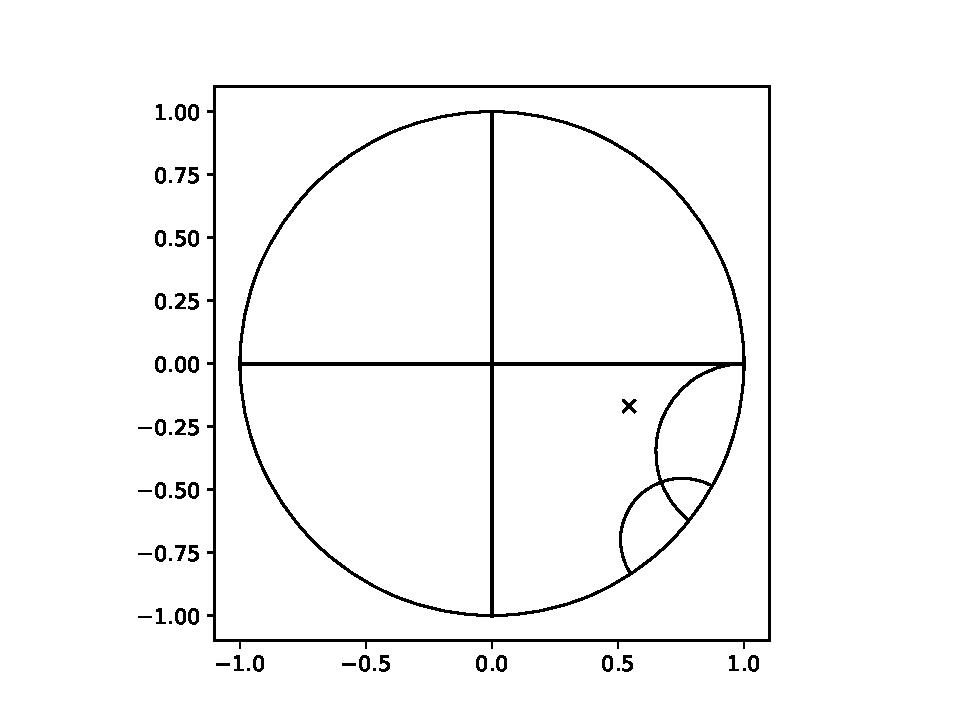
\includegraphics[trim=65 20 70 30, clip, width=0.6\linewidth]{F_r_disk.pdf}
	\caption{$\mathcal{F}_r$ in the disk}
	\label{FrDisk}
\end{figure}

\pagebreak

\subsection*{Choices of Test Points}
\begin{itemize}
	\item In the one version of the code which is working, we are using the cuspidal and flare expansions together; we use a set of test points obtained from each expansion
	\begin{itemize}
		\item We take half a horocycle at the height where $C$ intersects the fundamental domain in Figure \ref{FrWithCs}
		\item We take points on a ray out from the origin at a fixed angle and with radii between 1 and $\sqrt{\kappa}$ in Figure \ref{UFr}
	\end{itemize}
	\item The idea of admissible test points: call a point \textit{admissible} with respect to an expansion if it is in an area where the expansion is expected to converge quickly
	\begin{itemize}
		\item A point is admissible with respect to the cuspidal expansion if its height is above some fixed lower bound $y_0$
		\item A point is admissible with respect to the flare expansion if its angle is less that some fixed upper bound $\theta_0$
		\item A point is admissible with respect to the disk expansion if its radius is less than some fixed upper bound $\rho_0$
	\end{itemize}
	\item Ideas for the new algorithm which uses the disk and flare models together
	\begin{itemize}
		\item Keep the flare test points as they are, and replace the cuspidal test points with something which makes sense for the disk model
		\item Perhaps some points in the third and fourth quadrants at a fixed radius $\rho$, while allowing the angle $\theta$ to vary
	\end{itemize}
\end{itemize}

\section*{Questions for Andreas}

\begin{itemize}
	\item I noticed that you chose way more test points already in the chosen fundamental domain than outside of it.
	So most of the equations in the linear system are obtained by comparing the cuspidal expansion to the flare expansion (as opposed to comparing a single expansion to itself at two equivalent points).
	Do you have a heuristic reason for this decision?
	\item I noticed that when you chose your two sets of test points, you chose them to be very similar (i.e., very close together).
	I could see an argument for choosing the two sets much farther apart: that would make the linear systems look very different, so the only chance they should have of giving the same solution is when we input the true eigenvalue.
	I tried this, and it did not work as well.
	Do you have a heuristic reason for choosing these closer together?
	\item Generally, do you have any thoughts for tests that could be done to determine why the algorithm is failing in the disk case?
\end{itemize}

\section*{Ideas Sparked by the Meeting}

\begin{itemize}
	\item Andreas told us a heuristic idea for how he thinks about using different expansions
	\begin{itemize}
		\item Break the fundamental domain into finitely pieces such that, in each piece, we have chosen a ``best'' expansion for test points in that area
		\item Example: in a neighborhood of a flare, we could use a hyperbolic expansion, while in a neighborhood of a cusp, we could use a parabolic expansion
	\end{itemize}
	\item Recall Hejhal's idea for cutting down on computations: summing over a horocycle can pick out the $n^{th}$ Fourier coefficient (up to very small errors; see Booker-Str\"ombergsson-Venkatesh for a good discussion)
	\begin{itemize}
		\item Can doing the same thing in the flare and disk models save computation time?
		\item I think I already thought about this a while ago; problem is that we cannot compare expansions in this way
		\item Could still be useful to use this method for \textit{some} of the equations, while getting the rest of the equations by comparing expansions
	\end{itemize}
	\item Review previous work by K-S. Why are they only able to find 40ish decimal places?
	\begin{itemize}
		\item Check if computation of hypergeometric function is inaccurate to more decimal places (Str\"ombergsson made a note about this in his code)
		\begin{itemize}
			\item Maybe compare to Maple/Mathematica?
		\end{itemize}
		\item If not that, what else could it be? Think about how to determine this.
	\end{itemize}
	\item Try using all three expansions together in the Hecke group examples.
	\begin{itemize}
		\item This could be a useful test of the disk model
		\item Perhaps this could give faster convergence!
	\end{itemize}
	\item We could also start trying our algorithm out on a variety of examples
	\begin{itemize}
		\item McMullen 1998 discusses various examples in Section 3; I should take time to read through these examples
		\item One example which jumps out is a Schottky group with multiple flares and no cusps!
	\end{itemize}
	\item Moving up to hyperbolic 3-space
	\begin{itemize}
		\item Keep reading about 3-space with Brooke, since the eventual goal is to go up a dimension
		\item Could be interesting to move to 3-space soon and try examples which avoid the problems inherent in the Appolonian case (Kontorovich suggested an infinite volume fundamental domain with a bounding square)
	\end{itemize}
	\item Is there some way of capturing $L^2$ decay at the cusp without explicitly using the parabolic expansion?
	\begin{itemize}
		\item Perhaps some kind of sum across a horocycle?
		\item This seems to me to defeat the purpose of avoiding the cusp in computations, but I should think more about it
	\end{itemize}
\end{itemize}

\end{document}